Waste management is one of the most important issue in any country of the world. If not managed properly, it can threat the health and welfare of the general population.\\
\\
The key players that are responsible for the management of solid waste are the local governments of cities and provinces/states that handle this issue. The secondary players are Non-Governmental Organizations that also work in order to efficiently manage and recycle waste.\\
\\
This section will explore the methods as well as the technologies that have been used to identify and quantify garbage:\\
\\
Around the globe there are multiple technological platforms that exist which help and collaborate with these governments and/or Non-Governmental Organizations. Most of these platforms just use a simple complain system. Some examples are:
\section{Example Platforms:}
\subsection{Dallas sanitation service, 1800 recycle} are technological platforms that attempt to deal with the management of garbage by focusing on collection of garbage based on receiving requests.
\subsection{Rubicon} is another application which makes it easy to request garbage pickup service on the go, for a single location or many locations \cite{rubicon}.\\
\\
Another such example is GarbageCAN which works towards creating an app through which we can receive requests to collect recyclables that will be sold off to different recycling companies in the city.\\
\\
In terms of Pakistan not much work have been done towards the quantification and identification, however, Lahore Waste Management Company has launched an app called "Clean Lahore" which is also used to register different type of complains but none of these work on image processing and path optimization \cite{rizvi}.\\
\\
The government however has struggled with resources and has never implemented technology in this process.There are also many NGO's that operate within Pakistan that work on waste management. These mostly work in smaller scales with or without government collaboration. NGO's like WasteBusters are such examples that hire private cleaners to do this job.\\
\\
Now having discussed the generic technological innovation catering to the garbage crisis, we shall now discuss the efforts towards the identification and quantification of image using the analysis of image and employing computer vision techniques.
\section{Identification:}
\subsection{SpotGarbage} 
SpotGarbage is an example of an app which detects and coarsely segments garbage regions in a user-clicked Geo-tagged image \cite{mittal}. It is an application that we have tested out and are using for the identification segment of our project.
\section{Quantification:}
\subsection{Dimension of Object:}
Quantification requires volume estimation and there are different methods to extract 2 dimensions of any object from a 2D image if we have a reference object with its known dimensions.\\
\begin{figure}[!hb]
   \centering
   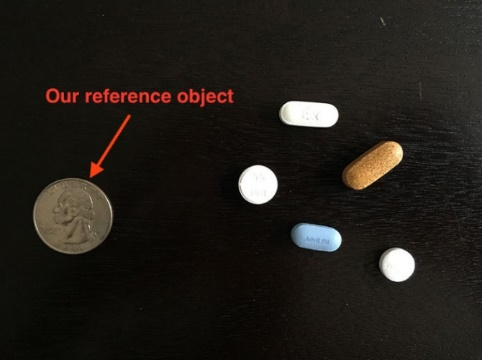
\includegraphics[scale=0.8]{images/q1.png}
   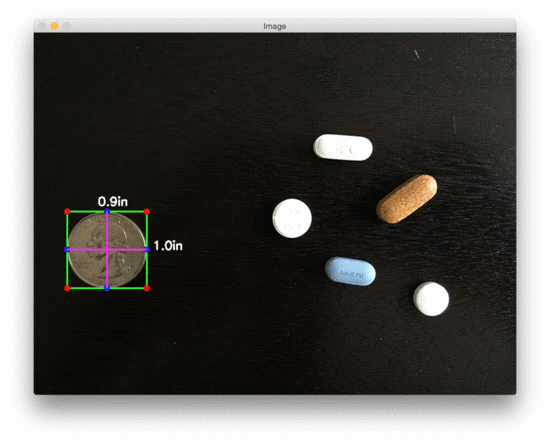
\includegraphics[scale=0.3]{images/q2.png}
   
   \caption{Dimensional Method}\label{fig:picture}
\end{figure}
\\
In the above figures there exists a reference object which is a coin whose 2 dimensions are known to us. Using that as a reference, we can calculate the dimensions of objects within the same frame. Now if another image is taken from a side angle ($90^{o}$ to the first image taken from the front angle) then we can also get 2 more dimensions. By this process we are getting the required dimensions to calculate an estimated volume of an object. However, as for the object of reference is concerned the drawback is there is a need of  reference object of known dimensions which could serve as reference for the mathematical model.
\subsection{Depth Analysis and Stereoscopic Vision:}
It uses two camera lenses, spaced slightly apart, to let the phone compare two images and piece together the depth of objects in stereo \cite{chaim}.\\
\\
The drawback of both the above mentioned techniques is that there are a lot of variables involved and that the camera particularly requires two lenses which becomes a pre-requisite for users when uploading an image to be identified or quantified but because of stereoscopic vision and depth analysis there are features that can be extracted which helps in estimating the distance between the camera and the object through which the size of the object can be estimated. \\
\\
\begin{figure}[!hb]
   \centering
   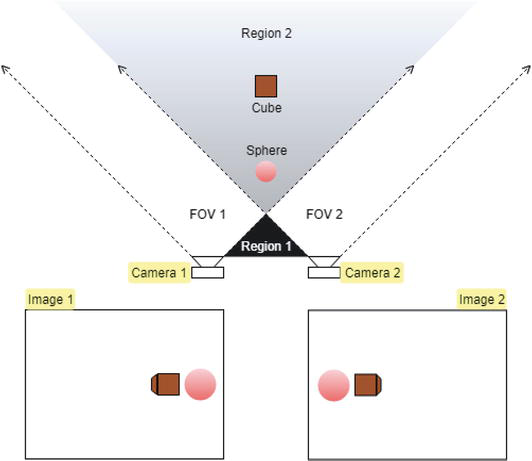
\includegraphics[scale=0.8]{images/q3.png}
   \caption{Depth Sensor/Stereoscopic Vision}\label{fig:picture}
\end{figure}
\\
This figure gives an idea of how things work. These techniques only work on stereo images from stereo cameras.
\subsection{3D Reconstruction from Multiple 2D Images:}
Another approach towards the quantification of garbage is 3D reconstruction from a single 2D image. Once we have a 3D model then the information about its volume can easily be obtained.\\
\\
Susheel, Suresh \cite{suresh} using images from 8 different perspectives were able to achieve an accuracy of 85 percent when quantifying using 3D Reconstruction. It utilized multiple 2D images from different angles on an object. Once we have those images then we can reconstruct an approximate 3D model from them.\\
\\
\begin{figure}[!hb]
   \centering
   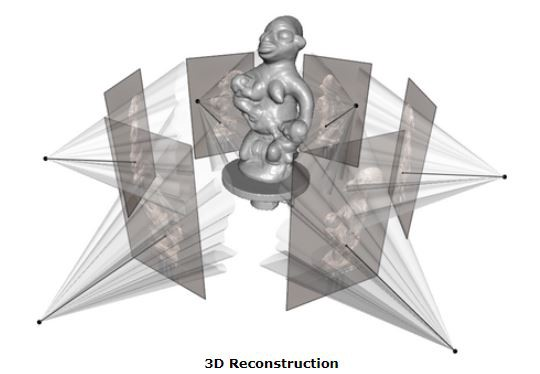
\includegraphics[scale=0.8]{images/q4.png}
   \caption{Dimensional Method}\label{fig:picture}
\end{figure}

The above mentioned figure is an example of 3D reconstruction where 6 2D images are being used.
The drawbacks of using techniques such as  3D reconstruction are 3D scanning, and the use of depth/range cameras are very costly and cumbersome to use.\\
\\
In order to improve this waste management as well as improve the communication gap present between both parties we wish to present a solution which uses images as well as locations to optimize waste collection and disposal.
\section{Object recognition}
Segmentation of garbage dumps from a scene.
Traditional approaches to segmentation, include image clustering. Image regions are clustered based on pixel intensities using an algorithm like Kmeans. This methodology would not work in our case because the region of interest (garbage dump), has varying pixel intensities in random distributions (very high spatial frequency). Also the number of clusters could not be fixed because the background would keep changing for every dump \cite{naik}\\
